\chapter[Medições Coletadas]{Medições Coletadas}\label{cap4}

Nessa sessão, será detalhada cada medição coledata nesse experimento, juntamente com o
objetivo.

\subsection{Medição 1}

A medição 1 é \textit{Estimar a o tamanho do desafio a ser implementado}. Consiste em pontuar, através do
scrum poker planner, o desafio proposto do ponto de vista do time do FF. Assim temos uma base para comparar a pespectiva do voluntário com
um valor base.

\begin{figure}[H]
  \centering
  \label{fig:indicadores}
  \includegraphics[keepaspectratio=true,scale=0.5]{figuras/medicao1.eps}
  \caption{Medicao 1}
\end{figure}

\subsubsection{Experimento}


Para realizar a bateria de testes foi definido um desafio, e a medicao um consistia-se em estimar a dificuldade desse desafio. O planejado era criar mais de um desafio, porém durante
a execução foi identificado que era necessário apenas um desafio, assim, não foi  preciso analisar a Medição 1.

\begin{figure}[H]
  \centering
  \label{fig:indicadores}
  \includegraphics[keepaspectratio=true,scale=0.4]{figuras/Challenge.eps}
  \caption{Desafio}
\end{figure}

\begin{figure}[H]
  \centering
  \label{fig:indicadores}
  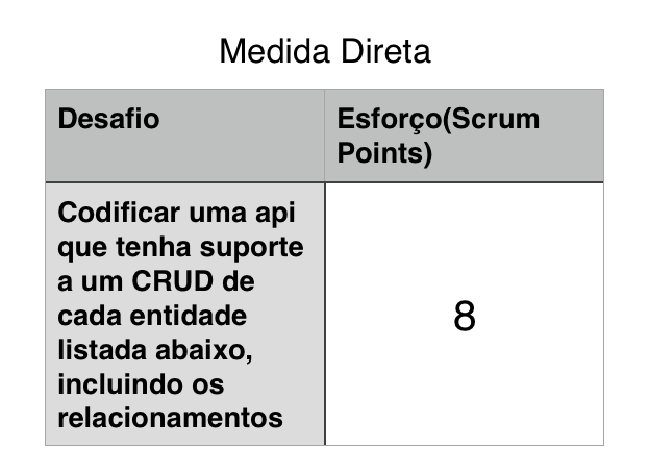
\includegraphics[keepaspectratio=true,scale=0.6]{figuras/Challenge_Scrum_Points.eps}
  \caption{Estimativa do desafio}
\end{figure}


\subsection{Medição 5}

A medição 5 é \textit{Estimar a experiência em desenvolvimento de serviços web dos desenvolvedores a serem recrutados para teste}. Consite em
atribuir um nível de conhecimento para cada vonlutário para nivelamento dos sub-grupos de teste.

\begin{figure}[H]
  \centering
  \label{fig:indicadores}
  \includegraphics[keepaspectratio=true,scale=0.7]{figuras/medicao5.eps}
  \caption{Medicao 5}
\end{figure}

\subsubsection{Experimento}

A medição 5 foi realizada através de um questionário, e calculando

\begin{figure}[H]
  \centering
  \label{fig:indicadores}
  \includegraphics[keepaspectratio=true,scale=0.6]{figuras/medicao5_meansure.eps}
  \caption{Medicao 5 Resultado}
\end{figure}

\subsubsection{Análise}
  Após a coleta das métricas os desenvolvedores com perfis para cada cenário foram idenfiticados,  selecionados e marcados em verde na tabela.

\subsection{Medição 2}

A medição 2 é \textit{Estimar a expectativa de tamanho da execução da atividade de criação de servidor com o framework}.
Consiste em pontuar, através do scrum poker planner, o desafio proposto do ponto de vista dos voluntários. Assim é possivel
comparar a grandeza do desafio do ponto de vista do voluntário para o time base do FF.

\begin{figure}[H]
  \centering
  \label{fig:indicadores}
  \includegraphics[keepaspectratio=true,scale=0.6]{figuras/medicao2.eps}
  \caption{Medicao 2}
\end{figure}

\subsubsection{Experimento}

A medição 2 foi realizada antes de cada bateria de testes

\subsubsubsection{Cenário 1}

\begin{figure}[H]
  \centering
  \label{fig:indicadores}
  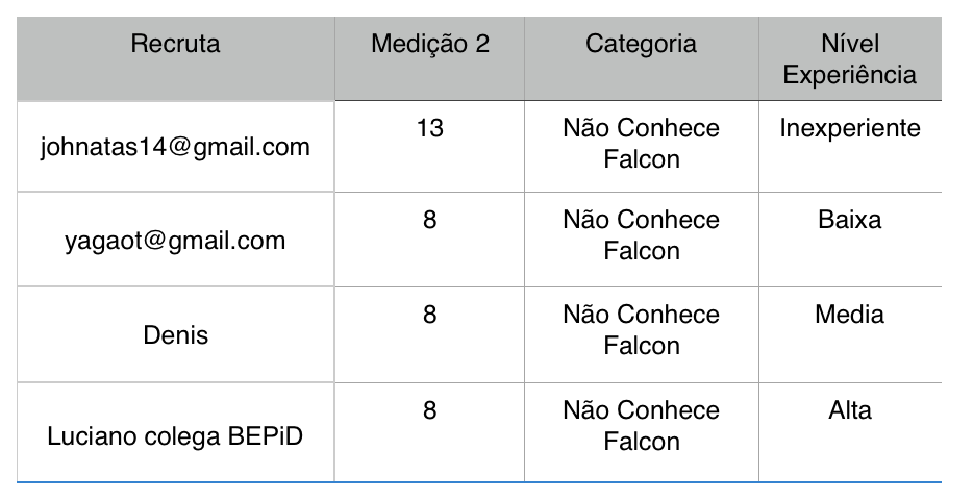
\includegraphics[keepaspectratio=true,scale=0.6]{figuras/Bateria1MEdicao2.eps}
  \caption{Bateria 1 Medicao 2 Resultado}
\end{figure}

\subsubsubsection{Cenário 3}

\begin{figure}[H]
  \centering
  \label{fig:indicadores}
  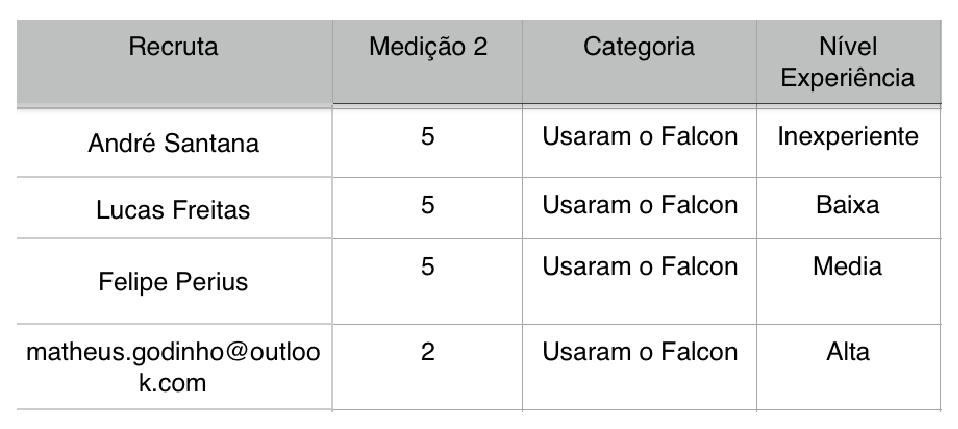
\includegraphics[keepaspectratio=true,scale=0.6]{figuras/Bateria3Medicao2.eps}
  \caption{Bateria 3 Medicao 2 Resultado}
\end{figure}



\subsubsection{Análise}
  A estimativa dos desenvolvedores foram menores após conhecerem o falcon, o que significa que o uso do falcon os deixam mais confiantes e torna o desafio mais fácil.



\subsection{Medição 3}

A medição 3 é \textit{Medir tempo da execução da atividade de criação de servidor com o framework}. Consistem em
coletar o tempo gasto por cada membro no desenvolvimento do desafio. Possibilitando o cálculo do custo como também
o da produtividade.

\begin{figure}[H]
  \centering
  \label{fig:indicadores}
  \includegraphics[keepaspectratio=true,scale=0.6]{figuras/medicao3.eps}
  \caption{Medicao 3}
\end{figure}

\subsubsection{Experimento}

A medição 2 foi realizada antes de cada bateria de testes

\subsubsubsection{Cenário 1}

\begin{figure}[H]
  \centering
  \label{fig:indicadores}
  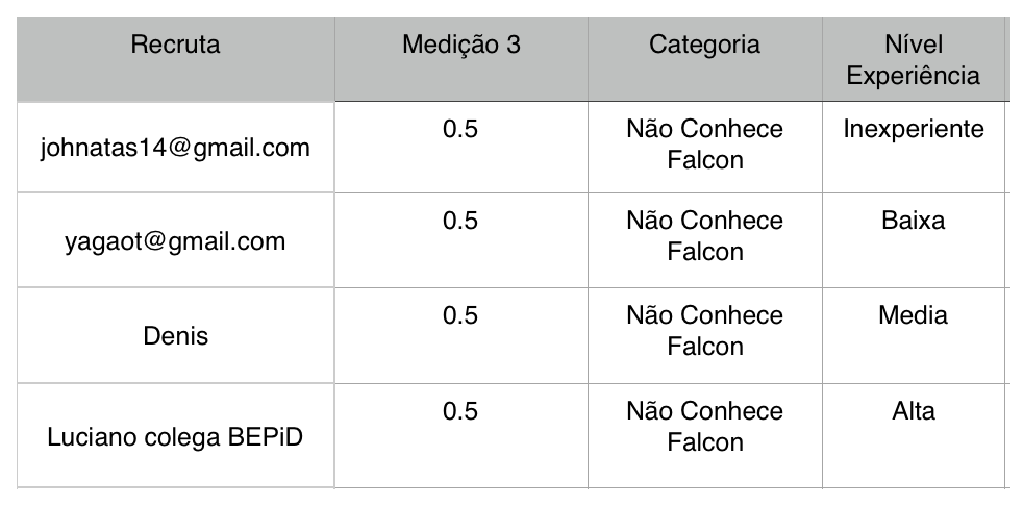
\includegraphics[keepaspectratio=true,scale=0.6]{figuras/Bateria1Medicao3.eps}
  \caption{Bateria 1 Medicao 3 Resultado}
\end{figure}

\subsubsubsection{Cenário 3}

\begin{figure}[H]
  \centering
  \label{fig:indicadores}
  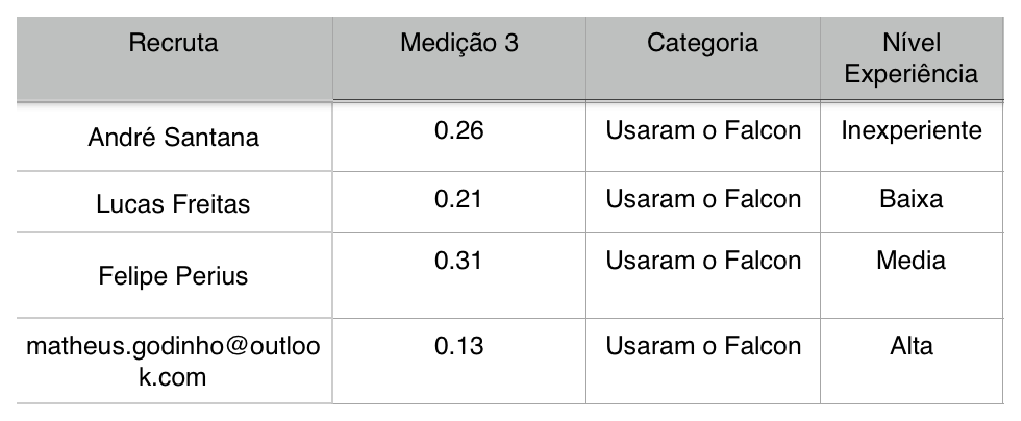
\includegraphics[keepaspectratio=true,scale=0.6]{figuras/Bateria3Medicao3.eps}
  \caption{Bateria 3 Medicao 3 Resultado}
\end{figure}



\subsubsection{Análise}

Foi constatado que a bateria de desenvolvedores que utilizaram o framework obtiveram um tempo menor do que os que não utilizaram.


\subsection{Medição 8}

A medição 8 é \textit{Estimar o número de erros gerados no desenvolvimento do desafio}. Consistem em
coletar o número de erros no desenvolvimento do desafio de cada membro. Possibilitando o cálculo da produtividade.

\begin{figure}[H]
  \centering
  \label{fig:indicadores}
  \includegraphics[keepaspectratio=true,scale=0.6]{figuras/Medicao8.eps}
  \caption{Medicao 8}
\end{figure}

\subsubsection{Experimento}

A medição 8 foi realizada após cada bateria de testes

\subsubsubsection{Cenário 1}

\begin{figure}[H]
  \centering
  \label{fig:indicadores}
  \includegraphics[keepaspectratio=true,scale=0.6]{figuras/Bateria1Medicao8.eps}
  \caption{Bateria 1 Medicao 8 Resultado}
\end{figure}

\subsubsubsection{Cenário 3}

\begin{figure}[H]
  \centering
  \label{fig:indicadores}
  \includegraphics[keepaspectratio=true,scale=0.5]{figuras/Bateria3Medicao8.eps}
  \caption{Bateria 3 Medicao 8 Resultado}
\end{figure}



\subsubsection{Análise}

Foi constatado que a bateria de desenvolvedores que utilizaram o framework obtiveram um número de erros menor do que os que não utilizaram.


\subsection{Medição 4}

A medição 4 é \textit{Estimar a produtividade dos desenvolvedores na execução da atividade de criação de servidor com o framework.}. Consiste
em cálcular a divisão do tamanho extimado pelo tempo gasto. Possibilitando a comparação da eficiência entre cada abordagem
na resolução do desafio.

\begin{figure}[H]
  \centering
  \label{fig:indicadores}
  \includegraphics[keepaspectratio=true,scale=0.6]{figuras/medicao4.eps}
  \caption{Medicao 4}
\end{figure}

\subsubsection{Experimento}

A medição 2 foi realizada antes de cada bateria de testes

\subsubsubsection{Cenário 1}

\begin{figure}[H]
  \centering
  \label{fig:indicadores}
  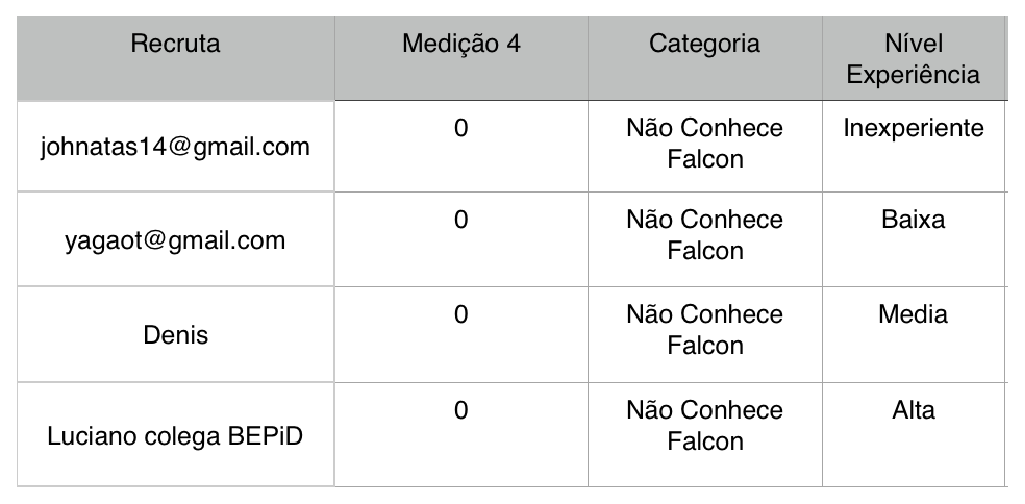
\includegraphics[keepaspectratio=true,scale=0.6]{figuras/Bateria1Medicao4.eps}
  \caption{Bateria 1 Medicao 4 Resultado}
\end{figure}

\subsubsubsection{Cenário 3}

\begin{figure}[H]
  \centering
  \label{fig:indicadores}
  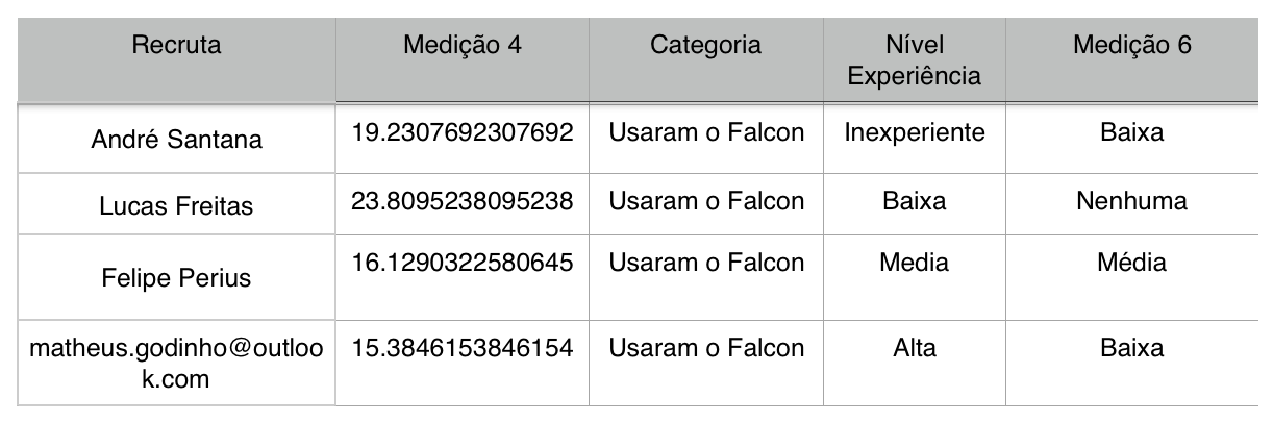
\includegraphics[keepaspectratio=true,scale=0.6]{figuras/Bateria3Medicao4.eps}
  \caption{Bateria 3 Medicao 4 Resultado}
\end{figure}



\subsubsection{Análise}

Foi constatado que a bateria de desenvolvedores que utilizaram o framework obtiveram um alto ganho de produtividade
em relação aos que não utilizaram o framework. Visto que, na primeira bateria de testes, nenhum dos membros conseguiu
terminar o desafio, já na bateria do cenário 3 todos os membros completaram com o sucesso o desafio, o que mostra o
aumento da produtividade do desenvolvedor.

\subsection{Medição 6}

A medição 6 é \textit{Estimar dificuldade de uso do produto gerado.} Consiste em validar a usabilidade do FF. Uma vez que
mesmo sendo eficiente do ponto de vista técnico não é usual.

\begin{figure}[H]
  \centering
  \label{fig:indicadores}
  \includegraphics[keepaspectratio=true,scale=0.6]{figuras/medicao6.eps}
  \caption{Medicao 6}
\end{figure}

\subsubsection{Experimento}

A medição 2 foi realizada antes de cada bateria de testes

\subsubsubsection{Cenário 1}

\begin{figure}[H]
  \centering
  \label{fig:indicadores}
  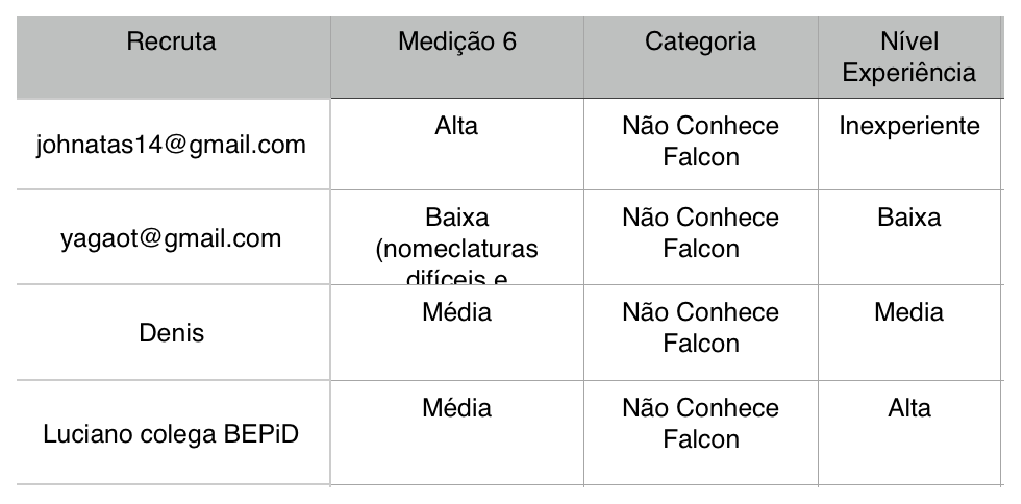
\includegraphics[keepaspectratio=true,scale=0.6]{figuras/Bateria1Medicao6.eps}
  \caption{Bateria 1 Medicao 6 Resultado}
\end{figure}

\subsubsubsection{Cenário 3}

\begin{figure}[H]
  \centering
  \label{fig:indicadores}
  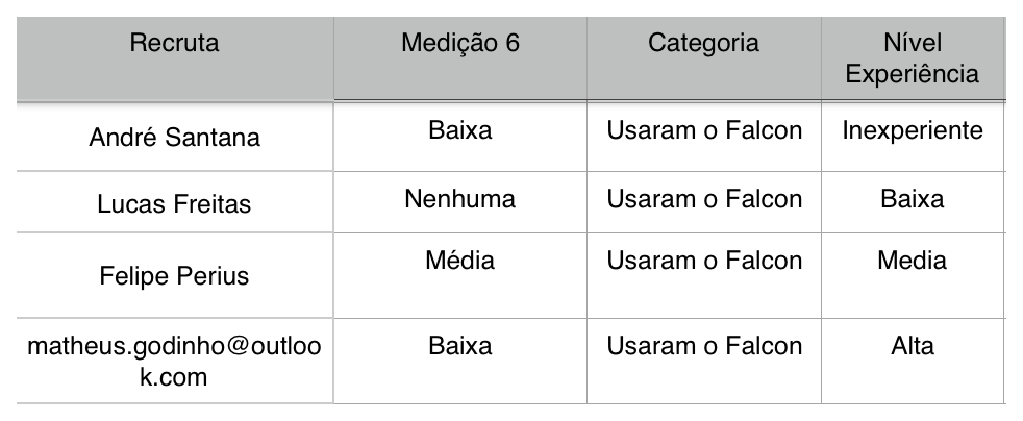
\includegraphics[keepaspectratio=true,scale=0.6]{figuras/Bateria3Medicao6.eps}
  \caption{Bateria 3 Medicao 6 Resultado}
\end{figure}


\subsubsection{Análise}

Foi constatado que na opinião dos desenvolvedores da bateria do cenário 3 o framework tem uma dificuldade de uso menor
do que outras plataformas utilizadas pelos desenvolvedores da bateria do cenário 1. E outra análise realizada
foi que a média de dificuldade do uso do framework na opinião de quem usou, é Baixa, o que mostra um ótimo resultado
em relação a usuabilidade.

\subsection{Medição 7}

A mediçnao 7 é \textit{Estimar a satisfação de uso do produto gerado.} Consiste em avaliar o interesse do voluntáo no FF, após
a sua utilização.

\begin{figure}[H]
  \centering
  \label{fig:indicadores}
  \includegraphics[keepaspectratio=true,scale=0.6]{figuras/medicao7.eps}
  \caption{Medicao 7}
\end{figure}

\subsubsection{Experimento}

A medição 2 foi realizada antes de cada bateria de testes

\subsubsubsection{Cenário 1}

\begin{figure}[H]
  \centering
  \label{fig:indicadores}
  \includegraphics[keepaspectratio=true,scale=0.6]{figuras/Bateria1Medicao7.eps}
  \caption{Bateria 1 Medicao 7 Resultado}
\end{figure}

\subsubsubsection{Cenário 3}

\begin{figure}[H]
  \centering
  \label{fig:indicadores}
  \includegraphics[keepaspectratio=true,scale=0.6]{figuras/Bateria3Medicao7.eps}
  \caption{Bateria 3 Medicao 7 Resultado}
\end{figure}



\subsubsection{Análise}

Foi constatado que na opinião dos desenvolvedores da bateria do cenário 3, usariam o framework novamente. E
75\% dos membros já queriam utilizar um beta da plataforma o quanto antes, o que mostra uma alta taxa de satisfação
do produto.

\section{Indicadores}

Uma vez que todas as medições forem coletadas, é necessario a definição de indicadores baseados nessas medições.
Nesses trabalho foram definidos e calculados quatro indicadores bases que são insumos para um indicador único que descreve
a operabilidade e a eficiência do FF, conforme a imagem \ref{fig:indicadores}. Sendo que cada indicador é representado por
um dos 3 números: -1, 0 e 1. O número -1 significa que o indicador não atingiu o resultado esperado e foi pior que o esperado,
o número 0 indica que o resultado foi indiferente, e por fim o número 1 indica que o objetivo foi atingido.

\begin{figure}[H]
  \centering
  \label{fig:indicadores}
  \includegraphics[keepaspectratio=true,scale=0.8]{figuras/i.eps}
  \caption{Composição do indicador}
\end{figure}

\subsection{Produtividade ganha com o uso do produto}

Esse indicador busca representar se a produtividade foi aumentada, reduzida ou não foi afetada. Esses casos são representados
respectivamente pelos números, 1, -1 e 0. O indicador foi gerado através da medição 4, que busca estimar a produtividade
dos desenvolvedores no desenvolvimento do desafio proposto, essa medição é gerada a partir das medições 2 e 3, que
são sobre tamanho e duração.

Na bateria 3, a qual foi utilizado o framework, foi observado, em todos os níveis de experiência, um aumento da
produtividade em relação aos desenvolvedores da bateria 1, a qual o desenvolvedor não utilizou o framework. Isso
mostra que o indicador foi positivo, isto é de valor igual a 1.

\begin{figure}[H]
  \centering
  \label{fig:indicador1}
  \includegraphics[keepaspectratio=true,scale=0.5]{figuras/indicadorProdutividade.eps}
  \caption{Geração do Indicador de Produtividade ganha com o uso do produto}
\end{figure}

\subsection{Satisfação do Usuário}

Esse indicador busca representar se a satisfação do usuário com o framework aumentou, diminuiu ou não foi afetada,
em relação ao uso de outras plataformas. Esses casos são representados respectivamente pelos números, 1, -1 e 0.
O indicador foi gerado através da medição 7, que busca medir a satisfação do usuário com o uso do produto.

Na bateria do cenário 3, a qual os desenvolvedores utilizaram o framework, em relação a bateria 1 foi observado que
a satisfação aumentou no nível inexperiente, diminuiu, no nível baixa e nos níveis média e alta, ela se manteve constante.
Com esses resultados o indicador total foi 0, visto que para um nível foi positivo, outro negativo e os outros dois
foram neutros.

\begin{figure}[H]
  \centering
  \label{fig:indicador1}
  \includegraphics[keepaspectratio=true,scale=0.5]{figuras/indicadorSatisfacao.eps}
  \caption{Geração do Indicador de Satisfação do Usuário}
\end{figure}

\subsection{Facilidade de Uso}

Esse indicador busca analisar e avaliar a usabilidade do produto em relação a outras plataformas, onde a usabilidade pode
ser considerada maior, menor, ou igual. Esses casos são representados respectivamente pelos números, 1, -1 e 0. O
indicador foi gerado através da medição 6, que busca medir a dificuldade de uso do produto.

Na bateria do cenário 3, a qual os desenvolvedores utilizaram o framework, em relação a bateria 1 foi observado que a
facilidade no uso do produto aumentou nos níveis inexperiente, baixa e alta, e se manteve constante no nível médio.
Com esses resultados o indicador total foi positivo, visto que em somente um nível a facilidade de uso não foi maior.

\begin{figure}[H]
  \centering
  \label{fig:indicador1}
  \includegraphics[keepaspectratio=true,scale=0.5]{figuras/indicadorFacilidadeUso.eps}
  \caption{Geração do Indicador de Facilidade de Uso}
\end{figure}
